% Provenance (never printed): see sources/outline_sources.md (Year 3: Gibbs
% energy and the phase rule in rocks, chemical potential recalled from the
% chemistry book; ternary diagrams; pseudosections, principle). Brief:
% sources/book5/BRIEFS.md, ch. 11. Curves from figdata/bachelor-3/
% gasp_tables.py, schreinemakers.py and regular_solution.py. Exercise and
% problem values in the Book 5 scratch calculator calc/ch11.py.
\chapter{Termodinâmica das rochas}\label{ch:b3:petrological-thermodynamics}

Uma granada de alguns milímetros de diâmetro cresceu zona por zona enquanto seu xisto era soterrado
e aquecido. Sua borda ainda registra, em seus teores de cálcio, ferro e magnésio, o último
equilíbrio que atingiu com a biotita e o plagioclásio ao seu redor. O volume do segundo ano
converteu essas composições em uma temperatura e uma pressão, com duas equações calibradas.
Este capítulo abre essa caixa-preta: de onde vêm as equações,
até onde se pode confiar nas tabelas de entalpias e entropias medidas,
quantos minerais uma rocha pode conter, como as soluções sólidas se misturam e
se separam, e como um computador transforma uma composição global em um mapa das
associações minerais que ela deveria exibir.

\begin{recall}
A energia de Gibbs, o potencial químico, a atividade e a constante de
equilíbrio, a variância e a regra das fases, a lacuna de miscibilidade e a
regra da alavanca estão nos volumes universitários dos livros de química. A reação univariante,
sua inclinação de Clapeyron $\Delta_rS/\Delta_rV$, o ponto invariante e o
diagrama de aluminossilicatos calculado a partir de tabelas está no volume do segundo ano, em seu
capítulo sobre fácies metamórficas; o geotermômetro e o geobarômetro, o
termômetro de troca granada--biotita e o barômetro GASP, em seu capítulo sobre
trajetórias P--T--t; diagramas ternários e a cotética, em seu capítulo sobre magmas. Uma
solução sólida e seus termos extremos estão no volume do primeiro ano, em seu capítulo sobre
minerais.
\end{recall}

\section{Equilíbrio a partir de tabelas}\label{sec:b3:petrological-thermodynamics:tables}

Para uma reação entre minerais de composição fixa, o equilíbrio na
temperatura $T$ e pressão $P$ ocorre quando $\Delta_rG(T, P) = 0$. As tabelas fornecem, a
\qty{298.15}{K} e \qty{1}{bar}, a entalpia de formação, a entropia e
o volume molar de cada mineral e a capacidade calorífica $C_p(T)$ acima. O
volume do segundo ano tratou $\Delta_rH$, $\Delta_rS$ e $\Delta_rV$ como constantes. O
resultado geral é o seguinte.

\begin{theorem}[Energia de Gibbs de uma reação em $T$ e $P$]\label{thm:b3:petrological-thermodynamics:dg}
Suponha-se que uma reação tenha, a $T_0 = \qty{298.15}{K}$ e \qty{1}{bar}, a
entalpia $\Delta_rH^\circ$ e entropia $\Delta_rS^\circ$, a
variação da capacidade calorífica $\Delta_rC_p(T)$ e, entre sólidos, uma variação de volume $\Delta_rV$
independente de $T$ e $P$. Então
\[
  \Delta_rG(T, P) = \Delta_rH^\circ + \int_{T_0}^{T}\Delta_rC_p\,\mathrm dT
  - T\Bigl(\Delta_rS^\circ + \int_{T_0}^{T}\frac{\Delta_rC_p}{T}\,\mathrm dT\Bigr)
  + (P - 1)\,\Delta_rV ,
\]
e a linha de equilíbrio é $P = 1 - \Delta_rG(T, 1)/\Delta_rV$.
\end{theorem}

\begin{proof}
A \qty{1}{bar}, $(\partial\Delta_rH/\partial T)_P = \Delta_rC_p$ e
$(\partial\Delta_rS/\partial T)_P = \Delta_rC_p/T$; integrando a partir de $T_0$
obtém-se $\Delta_rH(T)$ e $\Delta_rS(T)$, e $\Delta_rG = \Delta_rH -
T\Delta_rS$. Com $T$ fixo, $(\partial\Delta_rG/\partial P)_T = \Delta_rV$,
constante por hipótese; integrando de 1 a $P$ acrescenta-se $(P - 1)\Delta_rV$.
Fazendo $\Delta_rG(T, P) = 0$ obtém-se a linha.
\end{proof}

As duas integrais se cancelam em parte: sua soma é $\int_{T_0}^T\Delta_rC_p(1 -
T/T')\,\mathrm dT'$, na qual o fator $1 - T/T'$ é negativo e pequeno
onde $T'$ está próximo de $T$. Entre sólidos, $\Delta_rC_p$ é, por si só, pequeno,
porque a capacidade calorífica de um mineral é quase a soma das de seus
óxidos. A aproximação de propriedades constantes é, portanto, boa, e as
tabelas dizem quão boa ela é. Para a reação GASP,
\[
  \ce{3 CaAl2Si2O8 <=> Ca3Al2Si3O12 + 2 Al2SiO5 + SiO2},
\]
a tabela-resumo fornece $\Delta_rH^\circ = \qty{-36.3}{kJ}$,
$\Delta_rS^\circ = \qty{-130.7}{J.K^{-1}}$ e $\Delta_rV =
\qty{-6.61}{J.bar^{-1}}$, o que dá uma linha de inclinação \qty{19.8}{bar/K}; as
tabelas de alta temperatura, que incluem as capacidades caloríficas, fornecem
$\Delta_rG$ a cada \qty{100}{K}, e as duas linhas diferem em menos de
\qty{0.12}{kbar} até \qty{1200}{K} (a figura abaixo).
% ledger: rh95:gasp-298, rh95:gasp-ht

Os experimentos não concordam tão bem. Revertida em prensa de pistão-cilindro, a
900 e \qty{1250}{\celsius}, a reação fica \qty{0.9}{kbar} acima do previsto pelas
tabelas a \qty{627}{\celsius} e \qty{1.9}{kbar} acima a
\qty{927}{\celsius}. Com $\Delta_rV = \qty{-6.61}{J.bar^{-1}}$,
\qty{1.9}{kbar} equivale a um erro de \qty{12.6}{kJ} em $\Delta_rH$; as
incertezas das quatro entalpias de formação, \qty{3.2}{kJ} para
grossulária, \qty{2.0}{kJ} para anortita e cianita, \qty{1.0}{kJ} para
quartzo, combinam-se em cerca de \qty{8}{kJ} em $\Delta_rH$. A calorimetria fixa cada
mineral a alguns quilojoules; uma reação entre unidades de fórmula grandes multiplica
esses erros e os divide por uma pequena variação de volume.
% ledger: rh95:gasp-298, kn88:gasp

\begin{definition}[Conjunto de dados termodinâmicos internamente consistente]\label{def:b3:petrological-thermodynamics:dataset}
Um \emph{conjunto de dados termodinâmicos internamente consistente}\index{conjunto de dados termodinâmicos internamente consistente}
é uma tabela das propriedades padrão de
muitos minerais e fluidos (entalpia de formação, entropia, volume, capacidade
calorífica, expansão térmica e compressibilidade) ajustadas em conjunto, dentro
das incertezas da calorimetria, de modo que todo equilíbrio calculado a partir dela
passe pelos experimentos de reversão nos quais foi ajustado.
\end{definition}

Um conjunto desse tipo é ajustado uma única vez, por mínimos quadrados ponderados ou por
programação linear sobre todos os limites experimentais de uma vez, e depois usado em toda
reação entre seus minerais, incluindo reações nunca estudadas no
laboratório. Seus valores não são medidas independentes: uma entalpia pode
ser deslocada em um quilojoule para ajustar uma reação da qual participa. Valores de
conjuntos de dados diferentes jamais devem ser misturados.

\begin{omfigure}
\begin{tikzpicture}
\begin{axis}[omrecord, width=0.78\linewidth, height=0.5\linewidth,
  xlabel={temperatura (\unit{\celsius})}, ylabel={pressão (\unit{kbar})},
  xmin=400, xmax=1300, ymin=0, ymax=30, legend style={font=\scriptsize,
  at={(0.03,0.97)}, anchor=north west, legend cell align=left}]
% computed in figdata/bachelor-3/gasp_tables.py
\fill[omLithLime!60] (axis cs:900,19) rectangle (axis cs:1250,28);
\addplot[red!70!black, very thick] table[x=tc, y=p_kn88] {figdata/out/bachelor-3-gasp_tables-lines.dat};
\addlegendentry{experimento (termos extremos)}
\addplot[omDef, thick, densely dashed] table[x=tc, y=p_const] {figdata/out/bachelor-3-gasp_tables-lines.dat};
\addlegendentry{tabelas, $\Delta_rH$ e $\Delta_rS$ constantes}
\addplot[omDef, only marks, mark=*, mark size=1.8pt] table[x=tc, y=p_table] {figdata/out/bachelor-3-gasp_tables-tables.dat};
\addlegendentry{tabelas, com capacidades caloríficas}
\node[font=\scriptsize, align=center] at (axis cs:1075,26.3) {experimentos\\de reversão};
\node[font=\scriptsize] at (axis cs:560,4) {anortita};
\node[font=\scriptsize, align=center] at (axis cs:560,17) {grossulária + cianita\\+ quartzo};
\end{axis}
\end{tikzpicture}

\par\smallskip{\small A reação GASP de membros finais, 3 anortita = grossulária +
2 cianita + quartzo, calculada a partir das tabelas calorimétricas com propriedades
constantes (tracejada) e com as capacidades caloríficas (pontilhada), e a reta ajustada
aos experimentos de reversão feitos na faixa sombreada (vermelha, extrapolada abaixo de
\qty{900}{\celsius}).}\label{fig:b3:petrological-thermodynamics:gasp}
\end{omfigure}
% ledger: rh95:gasp-298, rh95:gasp-ht, kn88:gasp

\section{A regra das fases em rochas}\label{sec:b3:petrological-thermodynamics:phase-rule}

A regra das fases da química fornece a variância $F = c - p + 2$ de um sistema de
$c$ componentes em $p$ fases. Uma rocha é um sistema desse tipo, e seus minerais mostram
qual parte do plano pressão--temperatura ela atingiu o equilíbrio.

\begin{proposition}[Regra das fases mineralógica]\label{prop:b3:petrological-thermodynamics:goldschmidt}
Uma rocha que atingiu o equilíbrio a uma pressão e uma temperatura escolhidas
livremente dentro de uma área do plano pressão--temperatura apresenta no máximo tantas
fases quanto componentes: $p \le c$. Esta é a
\emph{regra das fases mineralógica}\index{regra das fases mineralógica}.
\end{proposition}

\begin{proof}
A regra das fases fornece $F = c - p + 2$ variáveis intensivas independentes. Se a
pressão e a temperatura podem variar ambas sem alterar a associação, duas delas são
livres: $F \ge 2$, logo $p \le c$. Uma rocha com $p = c + 1$ fases situa-se sobre uma
linha univariante; com $p = c + 2$, em um ponto invariante; nenhuma das duas situações é
provável para uma rocha coletada ao acaso.
\end{proof}

Uma rocha que viola a regra ou se equilibrou sobre uma linha de reação, o que suas texturas
podem revelar, ou nunca atingiu o equilíbrio como um todo: texturas de coroa,
minerais zonados e grãos reliquiares são causas comuns. A contagem de componentes
exige cuidado. Um componente presente apenas em uma fase de composição fixa, como
o zircão, pode ser descartado junto com essa fase; um componente fixado por um
reservatório externo, como a água quando um fluido percola a rocha, não é contado
como livre, visto que seu potencial químico é imposto.

Em torno de um ponto invariante, as linhas univariantes não se cruzam ao acaso. Em um
sistema de $c$ componentes, $c + 2$ fases se encontram no ponto, e $c + 2$
reações irradiam dele, cada uma escrita entre $c + 1$ fases e denominada pela
fase que omite, entre colchetes.

\begin{definition}[Análise de Schreinemakers]\label{def:b3:petrological-thermodynamics:schreinemakers}
A \emph{análise de Schreinemakers}\index{análise de Schreinemakers} é o método
que dispõe as linhas univariantes em torno de um ponto invariante a partir das
composições das fases apenas, antes de qualquer medida de suas propriedades
termodinâmicas: ela fixa a ordem das linhas, o lado de cada linha
que é estável, e as associações de cada setor entre elas.
\end{definition}

\begin{method}[Regras de Schreinemakers]\label{met:b3:petrological-thermodynamics:schreinemakers}
(1) Escreva as $c + 2$ reações, cada uma sem uma fase. (2) Cada linha é
estável de um lado do ponto e metaestável do outro. (3) A
extensão metaestável da linha ($i$), que omite a fase $i$, situa-se em um
setor onde $i$ é estável. (4) Nenhum setor entre duas linhas estáveis consecutivas
abrange mais de \ang{180}. (5) Através de uma linha, as associações de cada lado
são as dos dois lados de sua reação. Fixar uma linha com dados então
fixa todo o conjunto, a menos de uma imagem especular.
\end{method}

O ponto triplo dos alumino-silicatos do volume do segundo ano é o caso mais simples,
$c = 1$ e três linhas. A figura abaixo mostra um caso de dois componentes calculado
por \omterm{def:b3:petrological-thermodynamics:minimisation}{minimização da energia de Gibbs} em cada ponto.

\begin{omfigure}
\begin{tikzpicture}
\begin{axis}[omrecord, width=0.62\linewidth, height=0.5\linewidth,
  xlabel={temperatura (\unit{\celsius})}, ylabel={pressão (\unit{kbar})},
  xmin=400, xmax=800, ymin=1, ymax=9, grid=none]
% computed in figdata/bachelor-3/schreinemakers.py
\addplot[omDef, very thick] table[x=t, y=p] {figdata/out/bachelor-3-schreinemakers-ray_A_s.dat};
\addplot[omDef, thick, densely dashed] table[x=t, y=p] {figdata/out/bachelor-3-schreinemakers-ray_A_m.dat};
\addplot[omDef, very thick] table[x=t, y=p] {figdata/out/bachelor-3-schreinemakers-ray_B_s.dat};
\addplot[omDef, thick, densely dashed] table[x=t, y=p] {figdata/out/bachelor-3-schreinemakers-ray_B_m.dat};
\addplot[omDef, very thick] table[x=t, y=p] {figdata/out/bachelor-3-schreinemakers-ray_C_s.dat};
\addplot[omDef, thick, densely dashed] table[x=t, y=p] {figdata/out/bachelor-3-schreinemakers-ray_C_m.dat};
\addplot[omDef, very thick] table[x=t, y=p] {figdata/out/bachelor-3-schreinemakers-ray_D_s.dat};
\addplot[omDef, thick, densely dashed] table[x=t, y=p] {figdata/out/bachelor-3-schreinemakers-ray_D_m.dat};
\node[font=\scriptsize, fill=white, inner sep=1pt] at (axis cs:740,7.85) {(A)};
\node[font=\scriptsize, fill=white, inner sep=1pt] at (axis cs:540,8.75) {(C)};
\node[font=\scriptsize, fill=white, inner sep=1pt] at (axis cs:540,1.6) {(B)};
\node[font=\scriptsize, fill=white, inner sep=1pt] at (axis cs:740,2.15) {(D)};
\node[font=\scriptsize, align=center] at (axis cs:592,7.7) {A + B\\B + D};
\node[font=\scriptsize, align=center] at (axis cs:450,5.0) {A + D};
\node[font=\scriptsize, align=center] at (axis cs:592,2.4) {A + C\\C + D};
\node[font=\scriptsize, align=center] at (axis cs:765,5.0) {A + B\\B + C\\C + D};
\end{axis}
\end{tikzpicture}

\par\smallskip{\small Um conjunto de Schreinemakers em um sistema de dois componentes com
quatro fases de composições A (0), B ($1/3$), C ($2/3$) e D (1),
calculado para propriedades inventadas: linhas estáveis contínuas, extensões metaestáveis
tracejadas, e os pares estáveis em cada setor. (D) é A + C = 2B, (A) é B + D =
2C, (C) é 2A + D = 3B e (B) é A + 2D = 3C.}\label{fig:b3:petrological-thermodynamics:schreinemakers}
\end{omfigure}

\section{Soluções sólidas}\label{sec:b3:petrological-thermodynamics:solutions}

A maioria dos minerais formadores de rochas são soluções sólidas, e seus membros finais
aparecem nas reações por meio de suas atividades. O volume do segundo ano tomou $a = X^3$ para
a grossulária em uma granada e $a = X$ para a anortita em um plagioclásio.
Ambos são casos de um mesmo modelo.

\begin{definition}[Modelo de atividade de mistura em sítios]\label{def:b3:petrological-thermodynamics:site-mixing}
Em um \emph{modelo de atividade de mistura em sítios}\index{modelo de atividade de mistura em sítios}, os
íons de um mineral se misturam ao acaso em cada sítio cristalográfico, independentemente
dos demais sítios. A atividade ideal de um membro final é então o produto, sobre os
sítios, da fração de cada sítio que ele ocupa elevada ao número de
tais sítios por unidade de fórmula: $a_i = \prod_s X_{s,i}^{\,n_s}$.
\end{definition}

Uma granada $X_3Y_2\ce{Si3O12}$ tem três sítios dodecaédricos $X$ ocupados por
\ce{Ca}, \ce{Fe}, \ce{Mg} e \ce{Mn}: $a_{\text{grossular}} =
X_{\text{Ca}}^3$. Uma granada com $X_{\text{Ca}} = 0.10$ contém
\qty{10}{\percent} de grossulária, mas sua atividade é $10^{-3}$. O
modelo ideal conta as configurações; soluções reais também têm uma energia
de excesso, porque íons de tamanhos diferentes tensionam a rede.

\begin{definition}[Diagrama energia de Gibbs--composição]\label{def:b3:petrological-thermodynamics:gx}
Um \emph{diagrama energia de Gibbs--composição}\index{diagrama energia de Gibbs--composição}
representa, a temperatura e a pressão fixas, a energia de Gibbs molar de
cada fase de um sistema em função de sua composição. A paragênese estável de qualquer
composição global situa-se sobre o fecho convexo inferior das curvas: uma única fase
onde sua curva está sobre o fecho, e duas fases nas extremidades de uma tangente comum.
\end{definition}

\begin{proposition}[Solução regular]\label{prop:b3:petrological-thermodynamics:regular}
Em uma solução binária com um sítio de mistura por unidade de fórmula e
energia de interação $W$, a energia de Gibbs de mistura é
  \[
  G_{\text{mix}} = RT\bigl[x\ln x + (1 - x)\ln(1 - x)\bigr] + Wx(1 - x).
\]
Se $W > 0$, a solução é estável em toda composição acima de $T_c =
W/(2R)$; abaixo de $T_c$ a curva tem dois pontos de inflexão, e as composições
entre os dois pontos de sua tangente comum se separam em duas fases.
\end{proposition}

\begin{proof}
O primeiro termo é $-T$ vezes a entropia configuracional da mistura aleatória;
o segundo, a energia de excesso mais simples, simétrica e nula nas duas extremidades.
Derivando duas vezes, $G''_{\text{mix}} = RT/[x(1 - x)] - 2W$. Seu mínimo
em $x$ ocorre em $x = 1/2$, onde vale $4RT - 2W$, que é positivo para
todo $x$ se $T > W/(2R)$. Abaixo disso, $G''_{\text{mix}} < 0$ em um intervalo
em torno de $1/2$: a curva se encurva para baixo ali, uma reta entre dois pontos
da curva fica abaixo dela, e, pela definição acima, a rocha é de duas
fases.
\end{proof}

\begin{definition}[Solvus, exsolução]\label{def:b3:petrological-thermodynamics:solvus}
O \emph{solvus}\index{solvus} é a curva, no plano temperatura--composição,
que delimita a lacuna de miscibilidade de uma solução sólida: abaixo dela, um
único cristal de composição intermediária é instável e se divide em dois.
A \emph{exsolução (mineral)}\index{exsolução (mineral)} é essa divisão
dentro de um cristal durante o resfriamento: lamelas de uma composição crescem em um
hospedeiro da outra.
\end{definition}

Feldspatos alcalinos, piroxênios e anfibólios apresentam lamelas de exsolução,
visíveis ao microscópio ou a olho nu: a pertita de muitos granitos é
um feldspato alcalino exsolvido, um hospedeiro rico em potássio com
lamelas ricas em sódio. Entre o \omterm{def:b3:petrological-thermodynamics:solvus}{solvus} e o espinodal, onde $G''_{\text{mix}} = 0$,
um cristal precisa primeiro nuclear a segunda fase; dentro do espinodal, qualquer
pequena flutuação de composição cresce apenas por difusão.

\begin{omfigure}
\begin{tikzpicture}
\begin{groupplot}[group style={group size=2 by 1, horizontal sep=1.7cm},
  omrecord, width=0.47\linewidth, height=0.42\linewidth, title style={font=\small},
  legend style={font=\scriptsize, legend cell align=left}]
\nextgroupplot[title={(a) energia de Gibbs de mistura}, xlabel={$x$},
  ylabel={$G_{\text{mix}}$ (\unit{kJ.mol^{-1}})}, xmin=0, xmax=1, ymin=-9, ymax=1,
  legend style={at={(0.5,0.03)}, anchor=south}]
% computed in figdata/bachelor-3/regular_solution.py
\addplot[black, thick, densely dotted] table[x=x, y=g1500] {figdata/out/bachelor-3-regular_solution-gx.dat};
\addlegendentry{\qty{1500}{K}}
\addplot[red!70!black, thick, densely dashed] table[x=x, y=g1203] {figdata/out/bachelor-3-regular_solution-gx.dat};
\addlegendentry{$T_c = \qty{1203}{K}$}
\addplot[omDef, thick] table[x=x, y=g0900] {figdata/out/bachelor-3-regular_solution-gx.dat};
\addlegendentry{\qty{900}{K}}
\addplot[omDef, thin, forget plot] coordinates {(0.111,-0.635) (0.889,-0.635)};
\nextgroupplot[title={(b) solvus e uma seção em $X_0 = 0.3$}, xlabel={$x$},
  ylabel={temperatura (\unit{K})}, xmin=0, xmax=1, ymin=600, ymax=1300,
  legend style={at={(0.5,0.03)}, anchor=south}]
\addplot[omDef, thick] table[x=x, y=t_bin] {figdata/out/bachelor-3-regular_solution-solvus.dat};
\addlegendentry{solvus}
\addplot[black, thick, densely dotted] table[x=x, y=t_spin] {figdata/out/bachelor-3-regular_solution-solvus.dat};
\addlegendentry{espinodal}
\addplot[red!70!black, thick, forget plot] coordinates {(0.3,600) (0.3,1300)};
\addplot[red!70!black, thick, densely dashed] table[x=x2, y=t] {figdata/out/bachelor-3-regular_solution-section.dat};
\addlegendentry{isopletas em $X_0$}
\addplot[red!70!black, thick, densely dashed, forget plot] table[x=x1, y=t] {figdata/out/bachelor-3-regular_solution-section.dat};
\node[font=\scriptsize] at (axis cs:0.5,1250) {uma fase};
\node[font=\scriptsize] at (axis cs:0.5,950) {duas fases};
\end{groupplot}
\end{tikzpicture}

\par\smallskip{\small Uma solução regular com $W = \qty{20}{kJ.mol^{-1}}$
(ilustrativa). (a) Energia de Gibbs de mistura em três temperaturas; em
\qty{900}{K}, a tangente comum (linha fina) toca a curva em $x = 0.11$
e 0.89. (b) O \omterm{def:b3:petrological-thermodynamics:solvus}{solvus} e o espinodal; uma rocha de composição global $X_0 =
0.3$ (linha vertical vermelha) é uma fase acima de \qty{1136}{K} e duas fases
abaixo, cujas composições seguem o \omterm{def:b3:petrological-thermodynamics:solvus}{solvus} (tracejado).}\label{fig:b3:petrological-thermodynamics:solvus}
\end{omfigure}

\section{Pseudosseções}\label{sec:b3:petrological-thermodynamics:pseudosections}

O painel (b) da figura acima já é uma pequena \omterm{def:b3:petrological-thermodynamics:pseudosection}{pseudosseção}: para uma composição
global, ele indica quais fases são estáveis em cada temperatura, e quais são
suas composições e proporções. Uma rocha metamórfica tem cerca de dez
componentes e muitas soluções sólidas, mas o princípio é o mesmo.

\begin{definition}[Minimização da energia de Gibbs]\label{def:b3:petrological-thermodynamics:minimisation}
A \emph{minimização da energia de Gibbs}\index{minimização da energia de Gibbs} encontra, a
uma dada temperatura e pressão, o conjunto de fases, suas composições e
suas quantidades que minimiza a energia de Gibbs total de um sistema de
composição global fixa, sujeita à conservação de cada componente.
\end{definition}

\begin{definition}[Pseudosseção, isopleta, composição global efetiva]\label{def:b3:petrological-thermodynamics:pseudosection}
Uma \emph{pseudosseção}\index{pseudosseção} é um diagrama de fases, geralmente no
plano pressão--temperatura, calculado para uma composição global fixa: ele é
dividido em campos, cada um rotulado pela paragênese que minimiza a
energia de Gibbs ali. Uma \emph{isopleta (pseudosseção)}\index{isopleta (pseudosseção)}
é uma linha de uma pseudosseção ao longo da qual uma variável
composicional de uma fase, ou sua quantidade, é constante. A \emph{composição global
efetiva}\index{composição global efetiva} é a parte da composição da rocha que
ainda participa do equilíbrio, uma vez retirados os núcleos dos cristais zonados,
porfiroblastos isolados da matriz e outros materiais isolados
são removidos.
\end{definition}

Uma \omterm{def:b3:petrological-thermodynamics:pseudosection}{pseudosseção} não mostra linhas univariantes no sentido do volume do segundo
ano: em um sistema com soluções sólidas, a fronteira entre dois campos é
onde uma fase aparece ou desaparece, e sua posição depende da composição
global. Lê-se um desses diagramas de forma direta. A paragênese observada
fixa um campo; a composição medida de um mineral, por exemplo a de cálcio
na borda de uma granada, escolhe uma isopleta dentro dele; uma segunda isopleta,
de outro elemento ou de outro mineral, cruza-a na pressão e na temperatura
de equilíbrio. Granadas zonadas carregam uma sequência de cruzamentos desse
tipo, um para cada zona, ao longo da trajetória da rocha. Mas, à medida que
a granada cresce, seu núcleo retira manganês e cálcio do alcance da matriz:
a \omterm{def:b3:petrological-thermodynamics:pseudosection}{composição global efetiva} muda, e a \omterm{def:b3:petrological-thermodynamics:pseudosection}{pseudosseção} precisa ser recalculada
para as zonas mais tardias.

\begin{inthelab}[A bancada do petrologista]
\begin{minipage}[t]{0.55\linewidth}\vspace{0pt}
O petrologista estuda primeiro uma lâmina delgada ao microscópio petrográfico de
luz polarizada, para identificar a paragênese, suas texturas e quais grãos cresceram
juntos. A mesma lâmina, recoberta com carbono, vai então para uma microssonda
eletrônica, que mede a composição de pontos com alguns micrômetros de diâmetro
ao longo de perfis através das granadas. Um software que minimiza a energia de Gibbs,
com um \omterm{def:b3:petrological-thermodynamics:dataset}{conjunto de dados termodinâmicos internamente consistente} e um conjunto de modelos de atividade,
calcula uma \omterm{def:b3:petrological-thermodynamics:pseudosection}{pseudosseção} para a composição global, medida em uma fatia da mesma
rocha. As isopletas das composições medidas são traçadas sobre ela, e onde elas se cruzam
está a resposta. A incerteza do conjunto de dados e dos modelos de atividade,
e não a das medições, costuma limitá-la.
\end{minipage}\hfill
\begin{minipage}[t]{0.42\linewidth}\vspace{0pt}
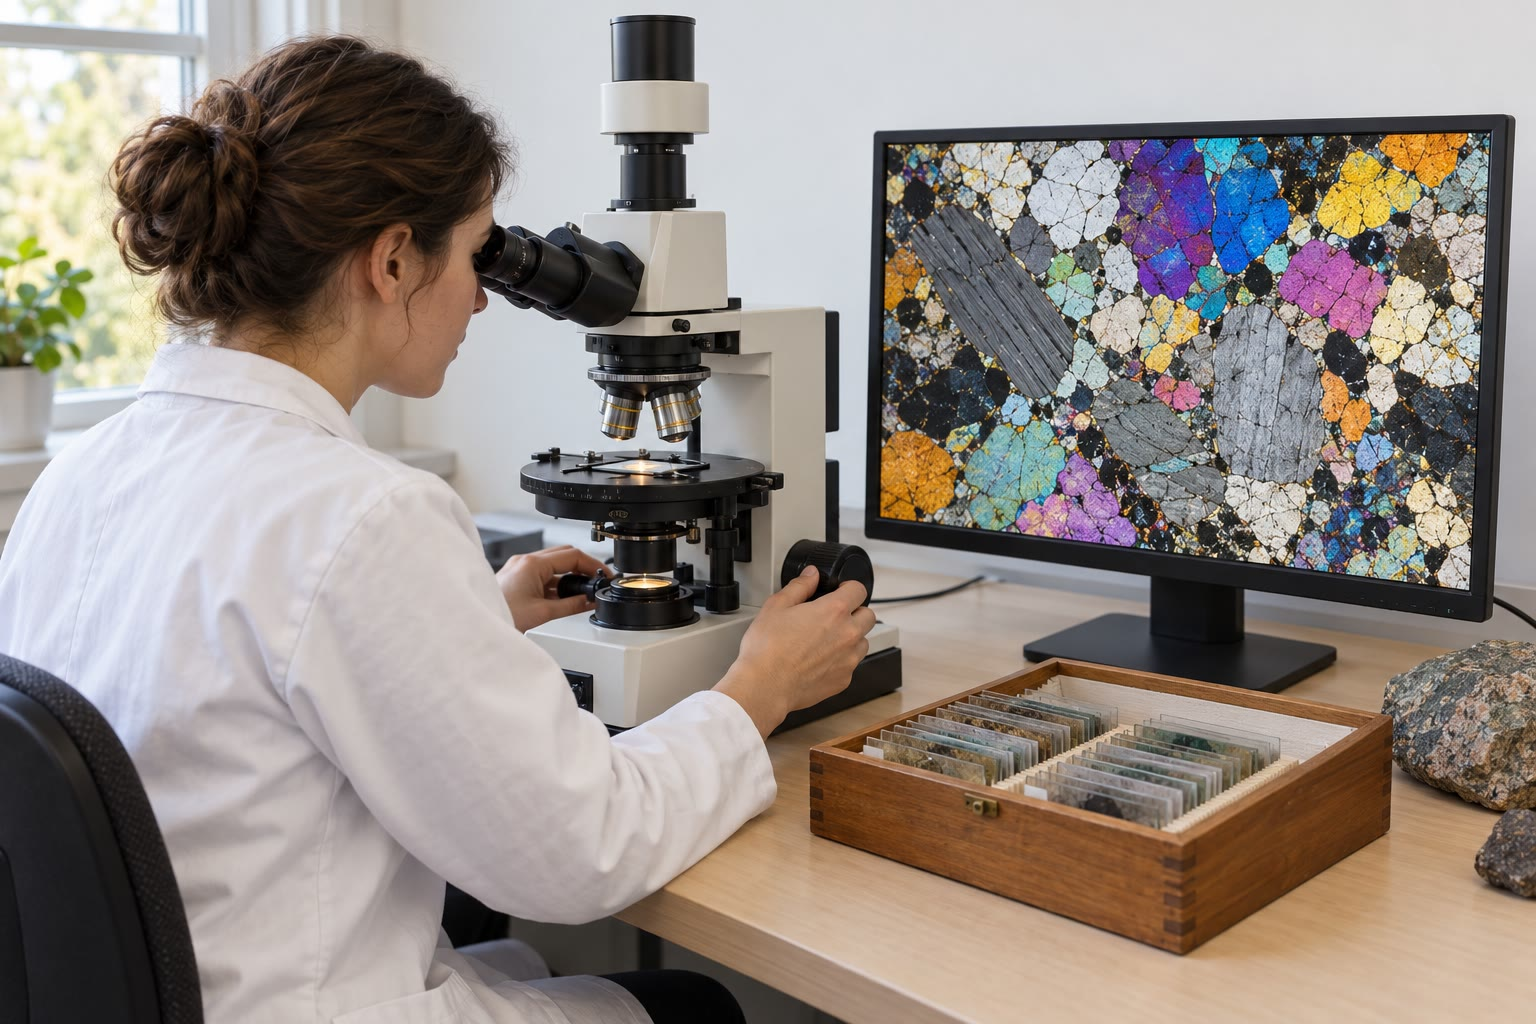
\includegraphics[width=\linewidth]{images/book5/ai/b3-petrology-desk.jpg}

{\scriptsize Um petrologista diante de um microscópio petrográfico, com uma caixa de
lâminas delgadas à mão e uma lâmina delgada em luz polarizada na tela
(Ilustração gerada por IA.)}
\end{minipage}
\end{inthelab}

\section{Exercícios}

\begin{exercise}[$\star$]\label{exo:b3:petrological-thermodynamics:1}
A partir das tabelas, a albita tem $\Delta_fH^\circ = \qty{-3935.0}{kJ}$, $S^\circ =
\qty{207.4}{J.K^{-1}}$, $V = \qty{100.07}{cm^3}$; jadeíta $-3029.3$, 133.5,
60.40; quartzo $-910.7$, 41.5, 22.69 (por mol). Para albita = jadeíta + quartzo,
calcule $\Delta_rH$, $\Delta_rS$, $\Delta_rV$ (em \unit{J.bar^{-1}}), a
inclinação de Clapeyron e a pressão da linha a \qty{600}{\celsius} com
propriedades constantes.
\end{exercise}
% ledger: rh95:ab-jd-qz

\begin{exercise}[$\star$]\label{exo:b3:petrological-thermodynamics:2}
Uma rocha do sistema \ce{MgO}--\ce{SiO2} contém forsterita, enstatita e
quartzo. Aplique a \omterm{prop:b3:petrological-thermodynamics:goldschmidt}{regra das fases mineralógica}. Qual é a conclusão?
\end{exercise}

\begin{exercise}[$\star$]\label{exo:b3:petrological-thermodynamics:3}
Calcule as atividades ideais de grossulária e piropo em uma granada com
$X_{\text{Ca}} = 0.20$ e $X_{\text{Mg}} = 0.15$, e de anortita em um
plagioclásio com $X_{\text{an}} = 0.40$ (um sítio).
\end{exercise}

\begin{exercise}[$\star$]\label{exo:b3:petrological-thermodynamics:4}
Calcule a temperatura crítica de uma solução regular com $W =
\qty{15}{kJ.mol^{-1}}$. Qual $W$ fornece $T_c = \qty{1000}{K}$?
\end{exercise}

\begin{exercise}[$\star\star$]\label{exo:b3:petrological-thermodynamics:5}
A \qty{1000}{K}, as tabelas fornecem as energias de Gibbs de formação
$-5432.2$ (grossulária), $-3478.1$ (anortita), $-2088.8$ (cianita) e $-730.2$
(quartzo), em \unit{kJ.mol^{-1}}. Calcule $\Delta_rG$ da reação GASP a
\qty{1}{bar} e sua pressão de equilíbrio, e compare com a linha experimental
$P_0 = 22.80\,T - 1093$ (bar, \unit{\celsius}).
\end{exercise}
% ledger: rh95:gasp-ht, kn88:gasp

\begin{exercise}[$\star\star$]\label{exo:b3:petrological-thermodynamics:6}
Para a solução regular da figura ($W = \qty{20}{kJ.mol^{-1}}$), calcule
$G_{\text{mix}}$ em $x = 0.5$ e \qty{900}{K}, depois no flanco do \omterm{def:b3:petrological-thermodynamics:solvus}{solvus} $x =
0.111$. Mostre que a separação de um cristal de composição 0.5 nos dois
flancos reduz sua energia de Gibbs, e em quanto.
\end{exercise}

\begin{exercise}[$\star\star$]\label{exo:b3:petrological-thermodynamics:7}
Quantas fases se encontram em um ponto invariante, e quantas linhas univariantes
irradiam dele, em um sistema de três componentes? No feixe da
figura, verifique que cada uma das quatro reações está balanceada.
\end{exercise}

\begin{exercise}[$\star\star$]\label{exo:b3:petrological-thermodynamics:8}
Uma rocha de composição global $X_0 = 0.3$ na solução regular da figura
resfriou-se a \qty{900}{K}, onde os flancos do \omterm{def:b3:petrological-thermodynamics:solvus}{solvus} são 0.111 e 0.889.
Calcule a proporção de cada fase.
\end{exercise}

\begin{exercise}[$\star\star$]\label{exo:b3:petrological-thermodynamics:9}
Com o barômetro GASP $P = P_0 + (3RT/6.21)\ln(X_{\text{Ca}}/X_{\text{an}})$
(bar), calcule $\partial P/\partial X_{\text{an}}$ a \qty{900}{K} e
$X_{\text{an}} = 0.30$. Em quanto um erro de 0.01 em $X_{\text{an}}$
desloca a pressão?
\end{exercise}

\begin{exercise}[$\star\star\star$]\label{exo:b3:petrological-thermodynamics:10}
Mostre que o espinodal de uma solução regular é $x(1 - x) = RT/(2W)$. A que
temperatura um cristal de composição 0.3 torna-se instável a qualquer pequena
flutuação, para $W = \qty{20}{kJ.mol^{-1}}$? Compare com a temperatura em que
ele atinge o \omterm{def:b3:petrological-thermodynamics:solvus}{solvus}, $T = W(1 - 2x)/[R\ln((1 - x)/x)]$, e explique
a diferença.
\end{exercise}

\begin{exercise}[$\star\star\star$]\label{exo:b3:petrological-thermodynamics:11}
Mostre que o \omterm{def:b3:petrological-thermodynamics:solvus}{solvus} de uma solução regular simétrica satisfaz $RT\ln[x/(1 -
x)] + W(1 - 2x) = 0$, e que ele atinge seu máximo, $T_c = W/(2R)$, em $x
= 1/2$.
\end{exercise}

\begin{exercise}[$\star\star\star$]\label{exo:b3:petrological-thermodynamics:12}
 Uma rocha contém \qty{2.0}{wt\percent} \ce{MnO}. Núcleos de granada contendo
 \qty{10}{wt\percent} \ce{MnO} constituem \qty{8}{wt\percent} da rocha e estão
 isolados da matriz. Calcule o teor de \ce{MnO} da
 \omterm{def:b3:petrological-thermodynamics:pseudosection}{composição global efetiva}. Por que isso importa para a \omterm{def:b3:petrological-thermodynamics:pseudosection}{pseudosseção} das bordas de granada?
\end{exercise}

\section{Problema: A granada do xisto de Varden}

\begin{problem}[{Problema de fim de semana --- a pressão e a temperatura de um
xisto fictício, a partir de tabelas, da regra das fases, dos modelos de atividade e
termobarometria}]
\label{pb:b3:petrological-thermodynamics:1}
% values: calc/ch11.py; gasp_tables.py
O xisto do embasamento das Varden Hills, metamorfizado há cerca de
\qty{480}{Ma} atrás, contém granada, biotita, muscovita, plagioclásio, cianita e
quartzo. Na borda de um cristal de granada e nos grãos ao redor dele, a microssonda
fornece: granada $X_{\text{Fe}} = 0.74$, $X_{\text{Mg}} = 0.12$, $X_{\text{Ca}} =
0.10$, $X_{\text{Mn}} = 0.04$; biotita $\ce{Mg}/(\ce{Mg} + \ce{Fe}) = 0.45$;
plagioclásio $X_{\text{an}} = 0.30$. Use as tabelas deste capítulo para a
reação GASP, o termômetro do volume do segundo ano
\[
T = \frac{52\,635 + 0.311P}{20.20 - 3R\ln K_D}\quad(T \text{ em K}, P
\text{ em bar}),
\]
e seu barômetro experimental $P = 22.80\,t - 1093 + (3RT/6.21)\ln
(X_{\text{Ca}}/X_{\text{an}})$, com $t$ em \unit{\celsius} e $T$ em
kelvin. Adote $R = \qty{8.314}{J.mol^{-1}.K^{-1}}$, uma densidade crustal de
\qty{2800}{kg/m^3} e $g = \qty{9.81}{m/s^2}$.

\medskip\noindent\textbf{Parte I --- As tabelas.}
\begin{enumerate}
  \item A partir da tabela-resumo, calcule $\Delta_rH^\circ$, $\Delta_rS^\circ$
        e $\Delta_rV$ da reação GASP.
  \item Calcule $\Delta_rG$ a \qty{298.15}{K} e \qty{1}{bar}. Qual dos lados
        é estável na superfície?
  \item Calcule a pressão do membro-final a \qty{900}{K} com
        propriedades constantes, e a inclinação de Clapeyron.
  \item As tabelas de alta temperatura fornecem $\Delta_rG = \qty{81.5}{kJ}$ a
        \qty{900}{K} e \qty{119.8}{kJ} a \qty{1200}{K} (\qty{1}{bar}).
        Calcule as pressões.
  \item Compare com a linha experimental nas mesmas temperaturas.
  \item Que erro em $\Delta_rH$ explicaria a discrepância a \qty{1200}{K}?
        Compare com a incerteza combinada das quatro entalpias.
  \item Por que as capacidades caloríficas alteram tão pouco o resultado?
\end{enumerate}

\medskip\noindent\textbf{Parte II --- A regra das fases.}
\begin{enumerate}[resume]
  \item Liste os componentes necessários para descrever os seis minerais e um
        fluido aquoso, e conte as fases.
  \item Calcule a variância com a regra das fases e verifique a \omterm{prop:b3:petrological-thermodynamics:goldschmidt}{regra
        das fases mineralógica}.
  \item Uma segunda amostra contém cianita e silimanita lado a lado. O que isso
        diz sobre a pressão e a temperatura?
  \item Água fluiu pela rocha durante o metamorfismo. Como isso
        altera a contagem?
\end{enumerate}

\medskip\noindent\textbf{Parte III --- Atividades e termobarometria.}
\begin{enumerate}[resume]
  \item Calcule as atividades ideais de grossulária e anortita, e $\ln K$
        da reação GASP na rocha.
  \item Calcule $K_D$ da troca granada--biotita.
  \item Calcule a temperatura a \qty{8}{kbar}.
  \item Calcule a pressão GASP nessa temperatura.
  \item Itere até a interseção das duas equações.
  \item Refaça a interseção com a linha do membro-final das tabelas, no lugar da
        linha experimental (com $\Delta_rV = \qty{-6.61}{J.bar^{-1}}$).
        Qual resultado você mantém, e por quê?
  \item De quanto um erro de 0.05 em $X_{\text{an}}$ desloca o
        resultado?
\end{enumerate}

\medskip\noindent\textbf{Parte IV --- O soterramento.}
\begin{enumerate}[resume]
  \item Com as propriedades constantes do volume do segundo ano, cianita =
        silimanita tem $\Delta_rH = \qty{7.7}{kJ}$, $\Delta_rS =
        \qty{12.6}{J.K^{-1}}$, $\Delta_rV = \qty{0.571}{J.bar^{-1}}$. O resultado está
        no campo da cianita?
  \item Calcule a profundidade de soterramento.
  \item O núcleo de granada tem $X_{\text{Ca}} = 0.07$ e cresceu com plagioclásio
        de mesmo $X_{\text{an}}$, em temperatura aproximadamente igual. O núcleo se
        formou mais fundo ou mais raso que a borda?
  \item Forneça a pressão de pico e a profundidade de soterramento do xisto de Varden.
\end{enumerate}
\end{problem}
